%%%%%%%%%%%%%%%%%%%%%%%%%%%%%%%%%%%%%%%%%%%%%%%%%%%%%%%%%%%%%%%%%
%%%		1 Aug 2014 (revised)                                      %%% 
%%%  see also                                                                             %%%
%%% http://ravirao.wordpress.com/2005/11/19/latex-tips-to-meet-publication-page-limits/  
%%%%%%%%%%%%%%%%%%%%%%%%%%%%%%%%%%%%%%%%%%%%%%%%%%%%%%%%%%%%%%%%%

\documentclass[11pt,a4paper]{article}
\usepackage{times}
\usepackage{fancyhdr}           % Allows better control over headers and footers
%\usepackage{layout}            % use with \layout to see the page layout for
%debugging purposes.
\usepackage[margin=2.5cm]{geometry}  %   set the margins using the
                                %   geometry package (which is much
                                %   the easiest way of doing this).
\usepackage[pdftex]{graphicx}   %   Pictures (means you have to
                                %   produce pdf output via pdflatex)
\usepackage[small,compact]{titlesec}   % Try to reduce the white space
                                % latex loves so much
\titlelabel{\thetitle. \quad}   % Reduce space around section heads
                                % and add a full stop after the number
\pagestyle{fancy}               % Invoke fancy headers

\renewcommand{\abstractname}{\vskip -5mm}  %  Change name of Abstract
                                %  to nothing and loose some of the
                                %  excessive white space
\begin{document}

\title{Ontology Verbalisation in isiZulu:\\ A Web Application Approach} \date{}
\author{Ngoni Choga\\ nickchoga@gmail.com
\and Ntokozo Zwane\\ ntkzwane@gmail.com
\and Paul Wanjohi\\ wnjpau001@alumni.uct.ac.za}

%%%  Set the headers via fancyhdr package
\lhead{OE Miniproject Report} % Short title for running head
\chead{}
\rhead{\date{}}   %  Fixed running head of the date
\lfoot{}
\cfoot{\thepage}    %  add page number as centre footer.
\rfoot{}
\renewcommand{\headrulewidth}{0.0pt}   % Don't want horizontal line
                                % under header.

\maketitle
\thispagestyle{plain}  % First page is plain style headings and
                       % footers (ie just the page number as footer).

\begin{abstract}
	Abstract here.
\end{abstract}

\section{Approach}


\subsection{Introduction}
\label{ss:introduction}

South Africa is a country that is known and celebrated for its diversity. 
With eleven official languages, South Africa provides a unique challenge 
for ontologists in particular when it comes to verbalising ontologies.
Chavula and Keet mention that most ontologies available are in 
English in particular the name of the ontology elements used. %\cite{} %TODO

Ontology verbalisation involves the construction of understandable sentences 
in a natural language. This implies that some translation and processing must
occur to convert an ontology from it ontology language to a natural language. 
As a result, ontology verbalisation would be classified into the natural 
language generation class of problems, a less notable subset of natural
language process than natural language understanding. %\cite{Rudnicky} %TODO

Since its inception, the Web Ontology Language (OWL) has had a lot research 
activity in the past decade that is geared towards allowing human users to 
view and edit OWL with much ease than dealing with raw code. Solutions 
constructed involve, the Manchester OWL syntax %\cite{Horridge} %TODO
and the graphical user interface Protege. %\cite{Knublauch}

The need for localisation of these ontologies becomes more relevant especially
when looking ontology users such as domain experts who seek to view and edit
these ontologies. A challenge still faced among common ontology languages. %\cite{Kaljurand}%TODO 

Attempts have been made to construct a solution to cater for specific natural 
languages. An example would include Attempto, which seeked to convert OWL 1.1 
ontologies to a controlled natural language Attempto Controlled English (ACE).
%\cite{Kaljurand}

Another notable example would be efforts made by Keet and Langa who were able
to create algorithms that would assist in the construction for an isiZulu 
grammar engine. They focus on the verbalisation of basic constructs need in
create an isiZulu grammar. %\cite{Keet, Langa}

In this paper, a review of research material into this problem will be made. 
Furthermore, algorithms selected for ontology verbalisation will be reviewed and
implemented. Finally, an inspection of the challenges encountered will be reviewed
and conclusions will be drawn in the end.

\subsection{Requirements Captured}

The next section deals with the analysis of your system. Cover the
functional, non-functional and usability requirements. This is where
you present your use case narratives and diagrams. 

Discuss the major analysis artefacts that you produced. We will expect
you to produce at least one overall description of the architecture
used in your system as a diagram, either here or below (see Section
\ref{ss:design-overview}). You may also want to include an analysis
class hierarchy diagram.

\subsection{Design Overview}
\label{ss:design-overview}

The next section is an overview of your design. The system design has
to be justified in terms of the expected behaviour of the final
product. 

If you produced a design class diagram put it here.

\begin{figure}[h!]
  \center{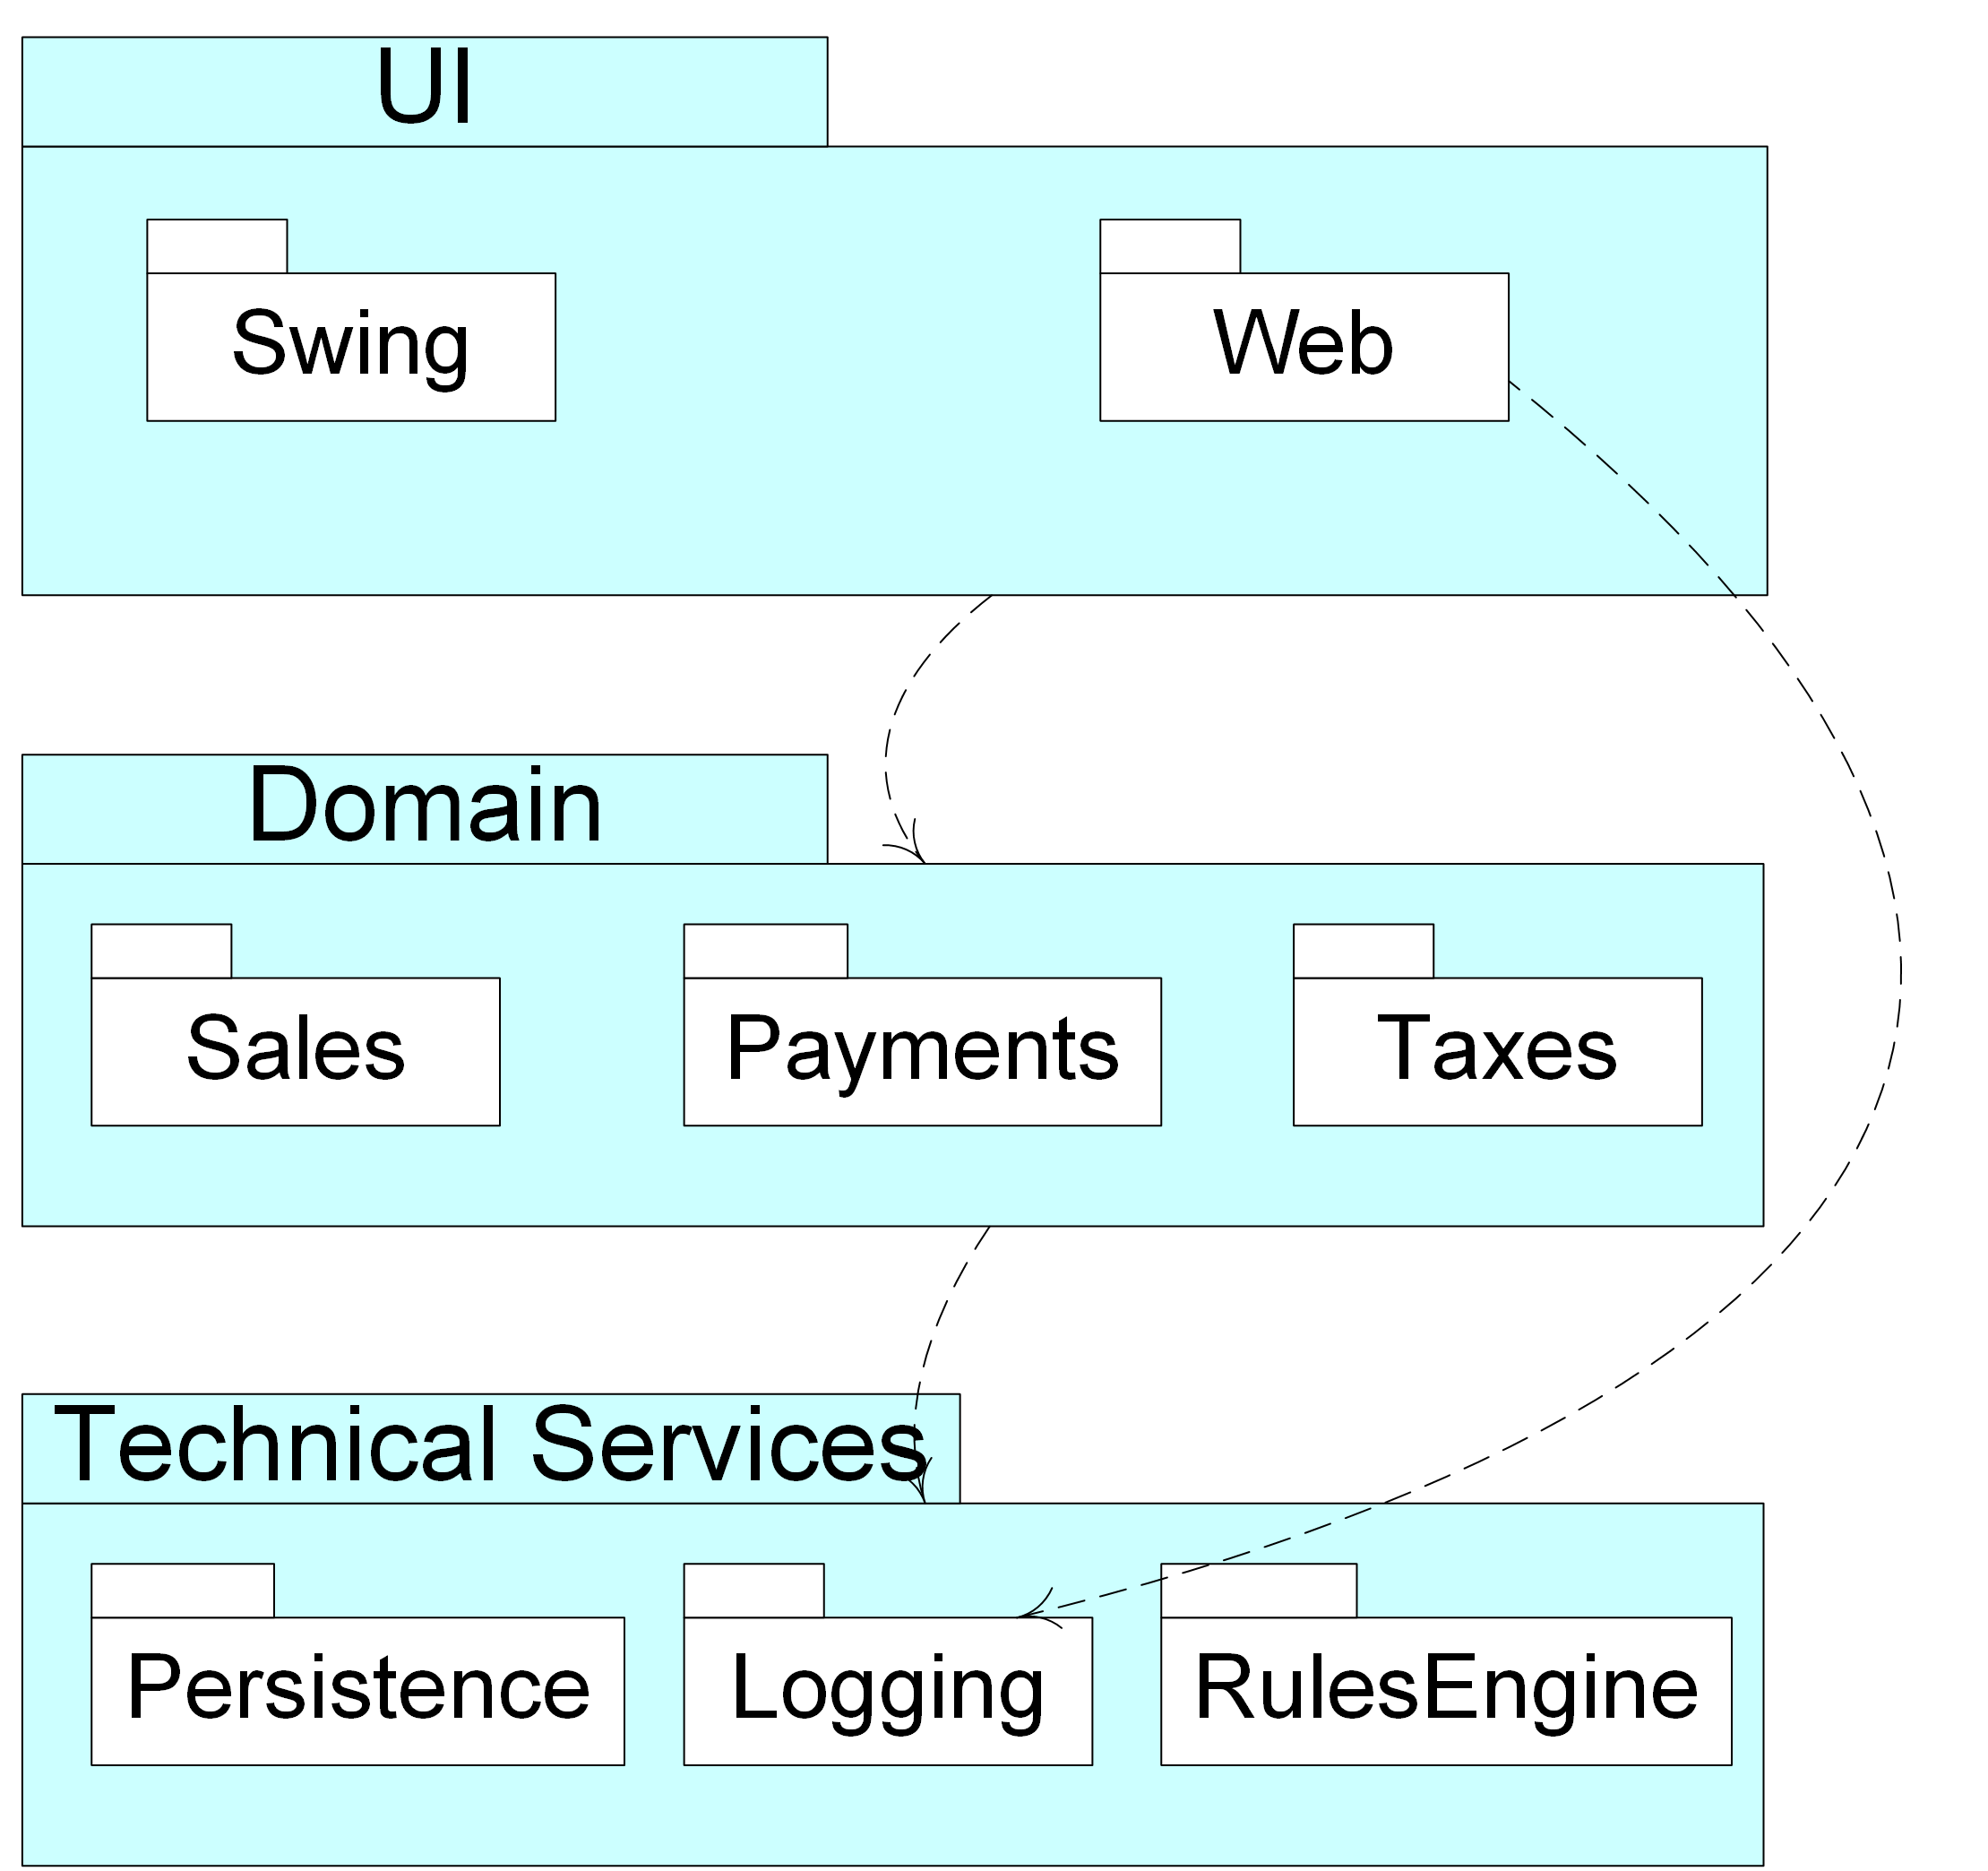
\includegraphics[scale=0.8]{architecture.png}}
  \caption{An architecture diagram. Caption to go below figure}
  \label{fig:architecture}
\end{figure}

You must present the overall architecture of the system together with
an architecture diagram. You may choose what kind of diagram best
suits your project but we would expect a layered architecture diagram
(see Figure \ref{fig:architecture}) unless there is a good reason for
some other kind of diagram. It need not be a formal UML diagram as
long as it conveys all the necessary information clearly.

You should then (in subsections) cover the algorithms and the data
organisation used and why they were considered the best. 

\subsection{Implementation}

Now we get to the details. 

\begin{itemize}
\item Describe your data structures and be sure to illustrate them
  with a diagram.

\item If your user interface was a key feature describe how that was
  implemented.

\item Discuss the function of the most significant methods in each
  class. This may well require flowcharts, or sequence diagrams, in
  some cases.

\item Any special relationship between the classes (e.g. friends) and
  why they exist.

\item A description of any special programming techniques or libraries
  used.
\end{itemize}

\subsection{Program Validation and Verification}
\label{ss:progr-valid-verif}

Tell us how you tested the system and why you believe it works.
Describe all the steps taken to validate the correctness of the
program.

If you had user tests then say what you did and what the results
were. Describe why these test data were chosen (what test conditions
the data was testing).  Table \ref{tab:tests} provides an example of
the sorts of results we are looking for. The full detail of the test
runs should be appended to the report.

\begin{table}[h!]
  \centering
\caption{A table of tests. A table caption goes above the table.}

  \begin{tabular}[t]{|p{5cm}|p{3cm}|p{3cm}|p{3cm}|} \hline \textbf{Data Set
    and reason for its choice} & \multicolumn{3}{c|}{\textbf{Test Cases}}\\
    \cline{2-4} & \emph{Normal Functioning} & \emph{Extreme boundary cases} &
    \emph{Invalid Data (program should not crash)} \\ \hline Preliminary test
    (see Appendix 3) & Passed & n/a & Fell over \\\hline &&&\\ \hline
    &&&\\ \hline
  \end{tabular}

\label{tab:tests}
\end{table}

Follow your table of results with a discussions of them highlighting
how useful and usable your system is for its intended purpose.

\subsection{Conclusion}
\label{ss:conclusion}

Your report must have a clear conclusion where you revisit the aims
set out in the beginning and discuss how well you met them. Did you
achieve the objective of creating a well-structured, modular, and
robust system?  Please summarize the design features and test results
that show this.

\subsection{User Manual}
\label{ss:user-manual}

Your system must have a user manual. Append this to your report (make
it Appendix A) or bind it separately if it is big. If your system is
interactive and has a good user interface with context dependent help
then this can be just a cheat sheet. Discuss the level at which your
user manual is to be pitched with your client. If your system is to be
extended then you might want to include a technical API manual.

\section{Conclusion}
\label{sec:conclusion}

This document has covered the major sections needed for your
report. You will probably have each of the subsections 2.1--2.7 as
major section in the report each with its own subsections. 

A marking guide for the report will be provided later.

\appendix
\section{Code Legibility and Output}

This is not strictly part of the report but is a requirement for the
final hand-in.

\begin{itemize}
\item Each method should start wide a brief description of its
  function.

\item Use indentation to display the structure within a method.

\item Comments should be used extensively. They are best used to
  describe logical blocks of code rather than individual
  statements. Line-by-line comments have the drawbacks of not
  providing any overview and of decreasing readability.

\item Meaningful identifiers should be chosen.

\item Output should be pleasingly formatted and easy to read.
\end{itemize}

You do, of course, have the option to call in any of your
favourite packages for setting maths, graphics, computer listings,
etc.

\begin{thebibliography}{9}

\bibitem[Kopka and Daly(2004)]{KopkaDaly}
Kopka, H. and Daly, P.W.  (2004) \textit{A Guide to \LaTeXe:
Document Preparation for Beginners and Advanced Users} (4th~edn).
Addison-Wesley.

\bibitem[Lamport(1994)]{Lamport}
Lamport L. (1994) \textit{\LaTeX: A Document Preparation System}
(2nd~edn). Addison-Wesley.

\bibitem[Mittelbach and Goossens(2004)]{Companion}
Mittelbach, F. and Goossens, M., (2004) \textit{The \LaTeX\
Companion} (2nd~edn). Addison-Wesley.

\end{thebibliography}
\end{document}
